\documentclass[letterpaper,10pt]{article}

%\setlength{\parindent}{0in}
%\usepackage{fullpage} 
\usepackage{amsmath}
\usepackage{amssymb}
\usepackage{enumerate}
\usepackage{graphicx}
\usepackage[table]{xcolor}
\usepackage{dcolumn}
\oddsidemargin 0.0in
\textwidth 6.5in
\newcolumntype{.}{D{.}{.}{-1}}
\newcommand*{\myalign}[2]{\multicolumn{1}{#1}{#2}}

%opening
\title{Assignment 1}
\author{Steve Mazza}
%\date{}

\begin{document}
\maketitle


\begin{frame}{Example of columns 1}
    \begin{columns}[c] % the "c" option specifies center vertical alignment
    \column{.5\textwidth} % column designated by a command
     Contents of the first column
    \column{.5\textwidth}
     Contents split \\ into two lines
    \end{columns}
\end{frame}
 
\begin{frame}{Example of columns 2}
     \begin{columns}[t] % contents are top vertically aligned
     \begin{column}[T]{5cm} % each column can also be its own environment
     Contents of first column \\ split into two lines
     \end{column}
     \begin{column}[T]{5cm} % alternative top-align that's better for graphics
          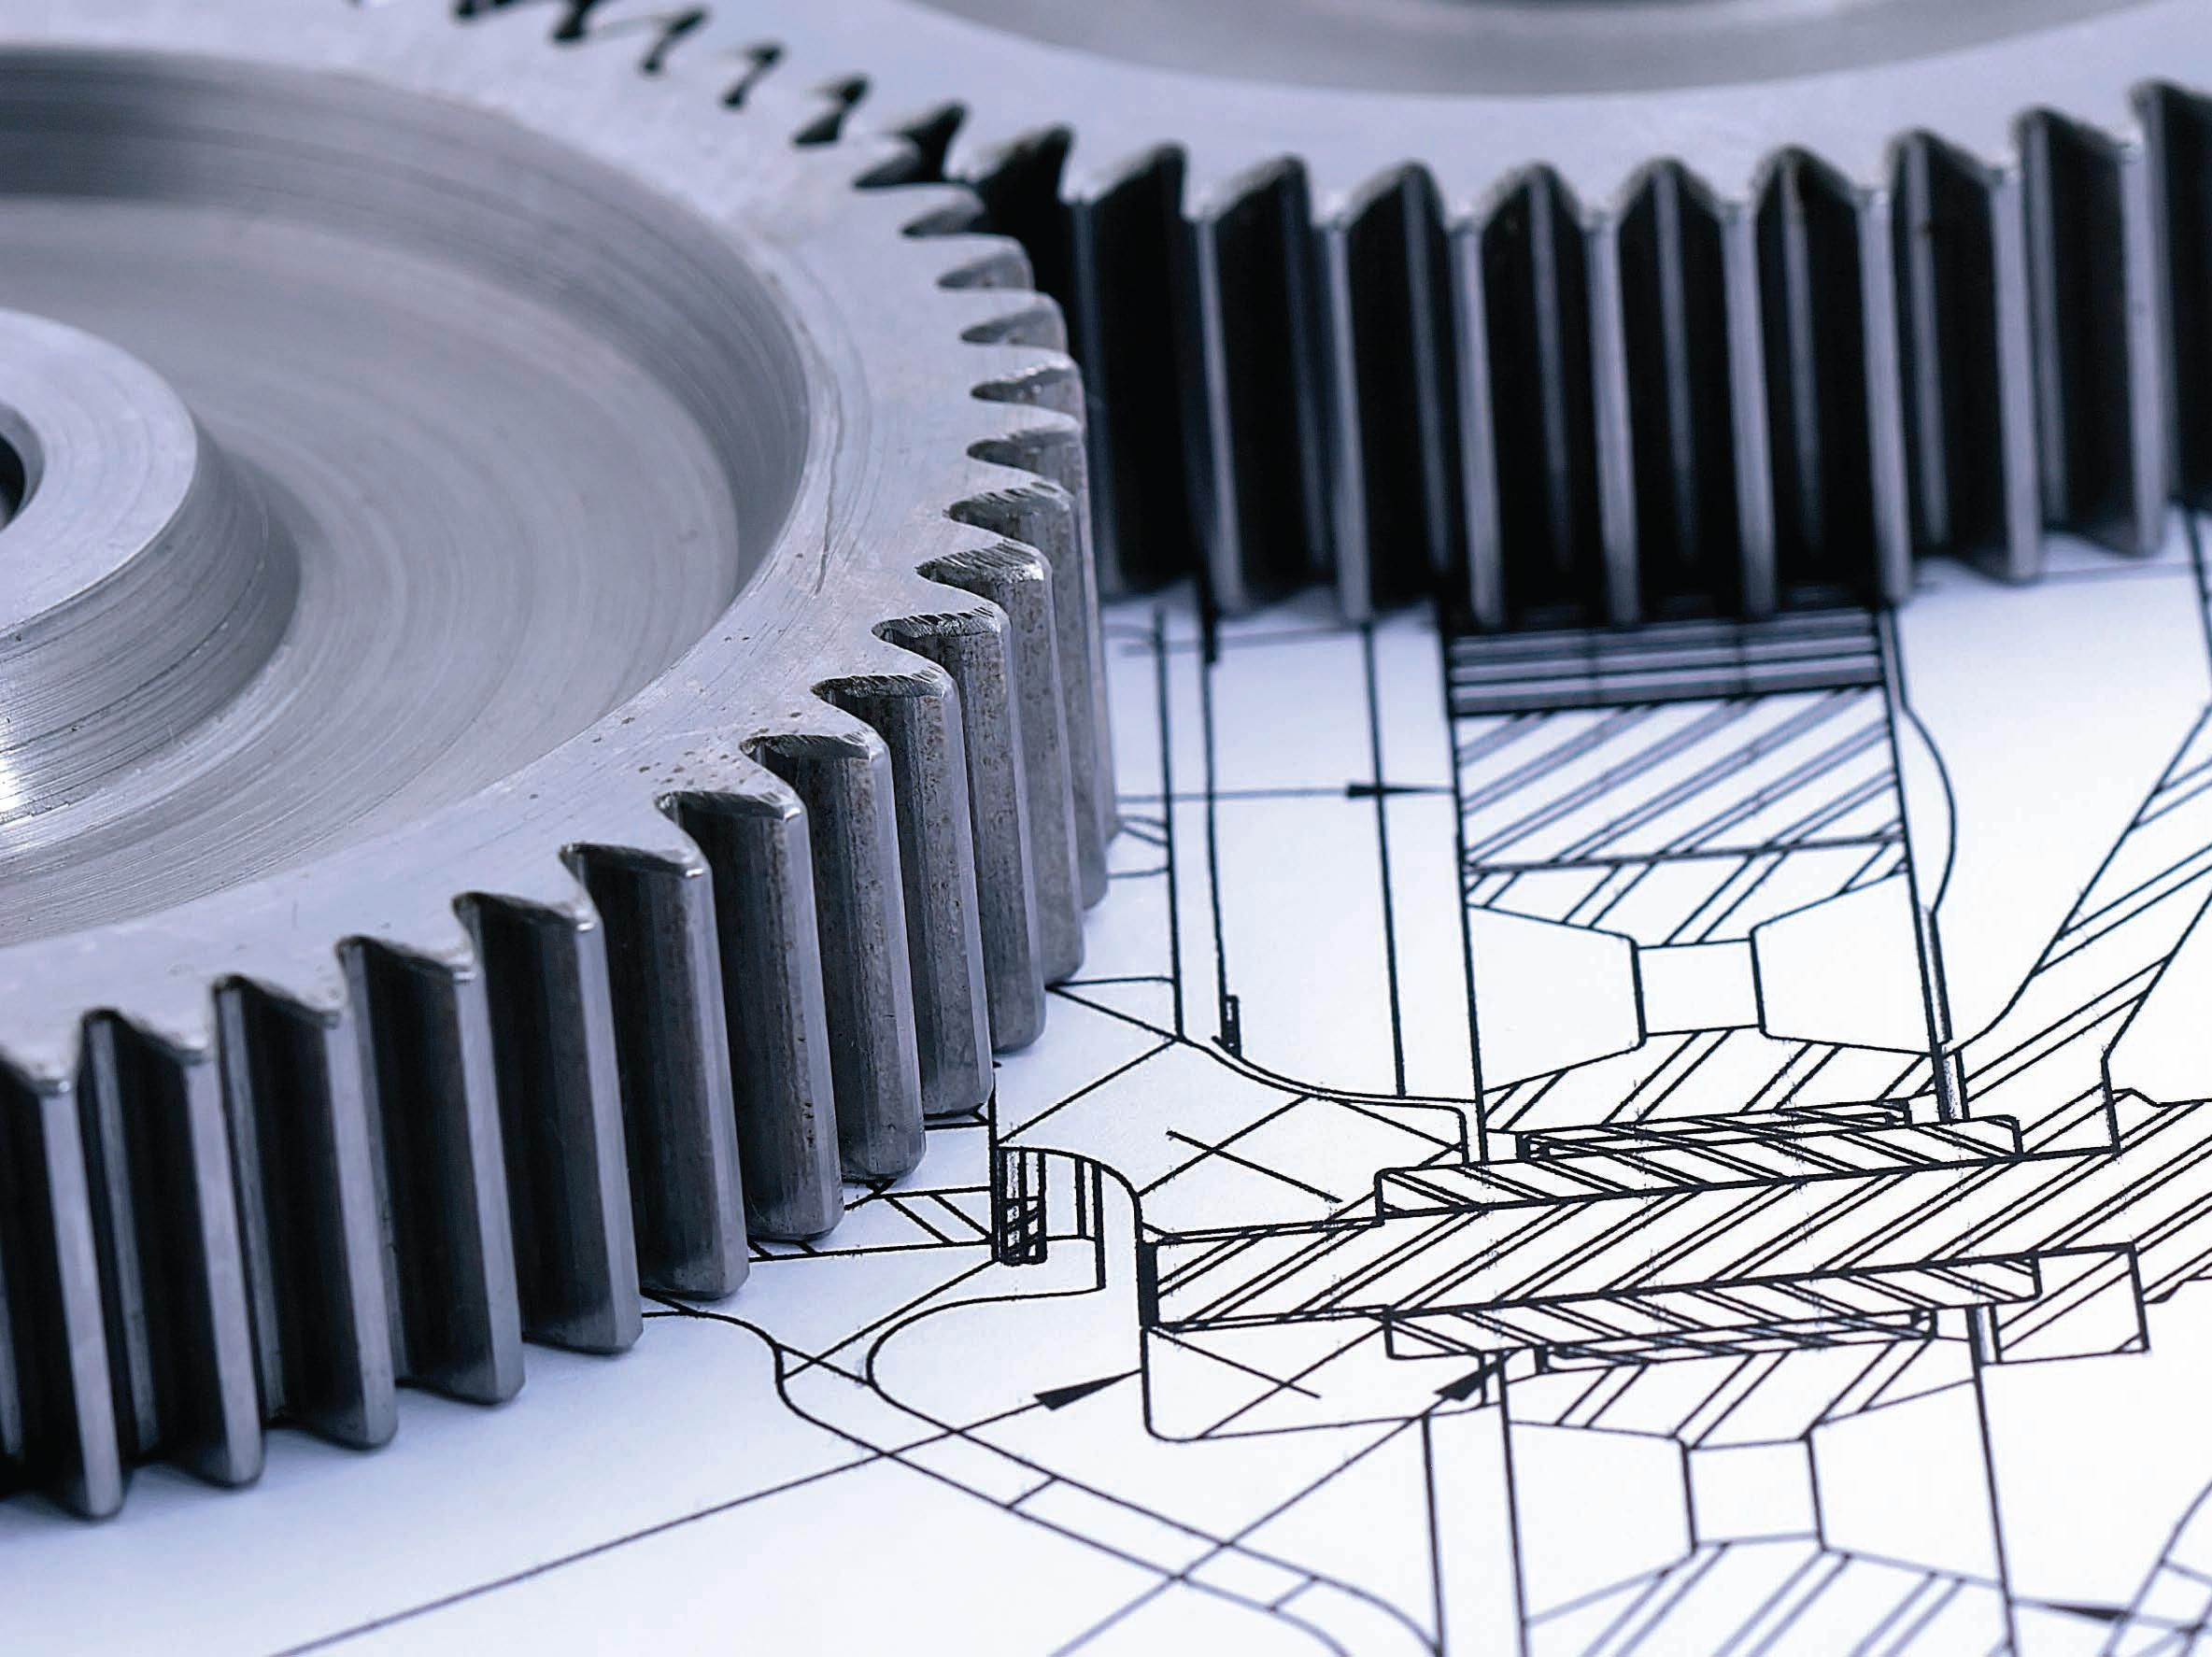
\includegraphics[height=3cm]{images/engineering.jpg}
     \end{column}
     \end{columns}
\end{frame}

\begin{frame}{Block Types}
   \begin{block}{This is a Block}
      This is important information
   \end{block}
 
   \begin{alertblock}{This is an Alert block}
   This is an important alert
   \end{alertblock}
 
   \begin{exampleblock}{This is an Example block}
   This is an example 
   \end{exampleblock}
\end{frame}

\end{document}
